\chapter{Dakota Tutorial}\label{tutorial}

\section {Quickstart}\label{tutorial:installation:quickstart}

This section provides an overview of acquiring and installing Dakota, 
running a simple example, and looking at the basic output available. 
More detailed information about downloads and installation can be found 
on the Dakota website \url{http://dakota.sandia.gov}.

\subsection {Acquiring and Installing Dakota}\label{tutorial:quickstart:installation}

Dakota operates on most systems running Unix or Linux operating
systems as well as on Windows, natively in a Command Prompt window,
and (optionally) with the help of a Cygwin emulation layer. Dakota
is developed and most extensively tested on Redhat Enterprise Linux
with GNU compilers, but additional operating systems
/ compiler combinations are tested nightly as well. See the Dakota
website for more information on supported platforms for particular
Dakota versions.

Department of Energy users: Dakota may already be available on your
target system. Sandia users should visit
\url{http://dakota.sandia.gov/} for information on supported Dakota
installations on engineering networks and cluster computers, as well
as for Sandia-specific downloads. At other DOE institutions, contact
your system administrator about Dakota availability. If Dakota is not
available for your target platform, you may still download Dakota as
described below.

New users should visit \url{https://dakota.sandia.gov/quickstart.html} to
gett started with Dakota. This typically involves the following steps:

\begin{enumerate}
  \item Download Dakota. \\
    You may download binary executables for your preferred platforms or 
    you can compile Dakota from source code. Downloads are available from 
    \url{http://dakota.sandia.gov/download.html}.
    
  \item Install Dakota. \\
    Instructions are available from 
    \url{http://dakota.sandia.gov/content/install-dakota}. Guidance is also 
    included in the Dakota source files, including
    \texttt{Dakota\_Source/INSTALL}. Further platform/operating system-specific
    guidance can be found in {\tt Dakota\_Source/examples/platforms}.

  \item Verify that Dakota runs. \\
    To perform a quick check that your Dakota executable runs, open a 
    terminal window (in Windows, cmd.exe), and type: \\
    \vspace{-2em}
    \begin{small}
    \begin{verbatim}
    dakota -v
    \end{verbatim}
      \end{small}
    \vspace{-2em}
    Dakota version information should display in your terminal window.
    For a more detailed description of Dakota command line options, see
    Section~\ref{tutorial:installation:running}.

  \item Participate in Dakota user communities. \\
    Join Dakota mail lists to get the most up-to-date guidance for
    downloading, compiling, installing, or running. For information about
    mail lists, getting help, and other available help resources, see \\
    \url{http://dakota.sandia.gov/content/get-help}.

\end{enumerate}

\subsection{Running Dakota with a simple input file}\label{tutorial:quickstart:running}
This section is intended for users who are new to Dakota, to demonstrate the basics 
of running a simple example. 

{\bf First Steps}
\begin{enumerate}
  \item Make sure Dakota runs. You should see Dakota version information
   when you type: \texttt{dakota -v}
  \item Create a working directory 
  \item Copy \texttt{rosen\_multidim.in} from the \texttt{Dakota/examples/users/}
    directory to the working directory -- see Section~\ref{intro:files} for help.
  \item From the working directory, run \texttt{dakota -i 
    rosen\_multidim.in -o rosen\_multidim.out > rosen\_multidim.stdout}
\end{enumerate}

{\bf What should happen} \\
Dakota outputs a large amount of information to help users track  progress. 
Four files should have been created:
\begin{enumerate}
  \item The screen output has been redirected to the file 
\texttt{rosen\_multidim.stdout}. \\
  The contents are messages from Dakota and notes about the 
progress of the iterator (i.e. method/algorithm).
  \item The output file \texttt{rosen\_multidim.out} 
contains information about the function evaluations.
  \item \texttt{rosen\_multidim.dat} is created due to the 
specification of \texttt{tabular\_graphics\_data} and \\
\texttt{tabular\_graphics\_file}. This summarizes 
the variables and responses for each function evaluation.
  \item \texttt{dakota.rst} is a restart file. If a Dakota 
analysis is interrupted, it can be often be restarted without 
losing all progress.
\end{enumerate}
In addition to the files, some plots are created due to the specification
of \texttt{graphics}. These can be helpful when processing the data or
diagnosing unexpected results.  If your particular installation or build
of Dakota does not support graphics, you will instead get a warning to
this effect.

Dakota has some data processing capabilities for output analysis. 
The output file will contain the relevant results. 
In this case, the output file has details
about each of the 81 function evaluations. 
For more advanced or customized data 
processing or visualization, the tabular data file can be imported into 
another analysis tool. 

{\bf What now?}
\begin{itemize}
  \item Assuming Dakota ran successfully, skim the three text files (restart files are in a binary format). These are described further in 
Section~\ref{tutorial:quickstart:output}.
  \item This example used a parameter study method, and the 
\texttt{Rosenbrock} test problem. More details about the example are in
Section~\ref{tutorial:examples:param_study} and the test problem is 
described in Sections~\ref{tutorial:examples:rosenbrock} and~\ref{additional:rosenbrock}.
  \item Explore the many methods available in Dakota in
    Chapters~\ref{ps}--~\ref{nls}.
  \item Try running the other examples in the same directory. These are mentioned
    throughout the manual and are listed in Table~\ref{tutorial:examples:table} 
    for convenience.
  \item Learn the syntax needed to use these methods. For help running Dakota, 
see Section~\ref{tutorial:installation:running} and for input file 
information, see Section~\ref{tutorial:dakota}. 
  \item Learn how to use your own analysis code with Dakota in Chapter~\ref{advint}.
\end{itemize}


\subsection {Examples of Dakota output}\label{tutorial:quickstart:output}
Beyond numerical results, all output files provide information that
allows the user to check that the actual analysis was the intended
analysis. More details on all outputs can be found in Chapter \ref{output}.

{\textbf{Screen output saved to a file}}

Whenever an output file is specified for a Dakota run, the screen
output itself becomes quite minimal consisting of version statements,
environment statements and execution times.

{\textbf{Output file}}

The output file is much more extensive, because it
contains information on every function evaluation (See Figure
\ref{tutorial:quickstart:rosenbrock_multidim:output}). It is 
organized into three basic parts:
\begin{enumerate}
\item Information on the problem
\begin{quote}
For this example, we see that a new restart file is being created
and Dakota has carried out a multidim\_parameter\_study with
8 partitions for each of two variables.
\end{quote}
\item Information on each function evaluation 
\begin{quote}
Each function evaluation is numbered. Details for function evaluation
1 show that at input variable values $x1= -2.0$ and $x2=-2.0$, 
the direct rosenbrock function is being evaluated.  There is one response
with a value of 3.609e+03.
\end{quote}
\item Summary statistics
\begin{quote}
The function evaluation summary is preceded by $<<<<<$. For this
example 81 total evaluations were assessed; all were new, none were
read in from the restart file. Correlation matrices complete the statistics
and output for this problem. Successful runs will finish with
$<<<<<$ Iterator {\it study\_type} completed.
\end{quote}
\end{enumerate}

{\textbf{Tabular output file}}

For this example, the default name for the tabular output file 
\texttt{dakota\_tabular.dat} was changed in the input file to
\texttt{rosen\_multidim.dat}. This tab-delimited text file
(Figure \ref{tutorial:quickstart:rosenbrock_multidim:dat})
summarizes the inputs and outputs to the function evaluator.
The first line contains the names of the variables and responses: 
\newline
\begin{tabular}{llll}
\%eval\_id           &  x1  &           x2&  response\_fn\_1 \\
\end{tabular}
\newline
The number of function evaluations will match the number of 
evaluations listed in the summary part of the output file for
single method approaches; the
names of inputs and outputs will match the descriptors 
specified in the input file. This file is ideal for import into
other data analysis packages.


\begin{figure}[ht!]
  \centering
  \begin{bigbox}
    \begin{small}
      \begin{verbatim}
{Writing new restart file dakota.rst
methodName = multidim_parameter_study
gradientType = none
hessianType = none

>>>>> Running multidim_parameter_study iterator.

Multidimensional parameter study for variable partitions of
                                     8
                                     8


------------------------------
Begin Function Evaluation    1
------------------------------
Parameters for function evaluation 1:
                     -2.0000000000e+00 x1
                     -2.0000000000e+00 x2

Direct function: invoking rosenbrock 

Active response data for function evaluation 1:
Active set vector = { 1 }
                      3.6090000000e+03 response_fn_1
.
.
.
<<<<< Function evaluation summary: 81 total (81 new, 0 duplicate)

Simple Correlation Matrix among all inputs and outputs:
                       x1           x2 response_fn_1 
          x1  1.00000e+00 
          x2  1.73472e-17  1.00000e+00 
response_fn_1 -3.00705e-03 -5.01176e-01  1.00000e+00 
. 
.
.
<<<<< Iterator multidim_parameter_study completed.}
\end{verbatim}
    \end{small}
  \end{bigbox}
\caption{Rosenbrock 2-D parameter study example: excerpt from output file}
\label{tutorial:quickstart:rosenbrock_multidim:output}
\end{figure}


\begin{figure}[ht!]
  \centering
  \begin{bigbox}
    \begin{small}
      \begin{verbatim}
%eval_id          interface               x1             x2  response_fn_1 
       1              NO_ID               -2             -2           3609 
       2              NO_ID             -1.5             -2         1812.5 
       3              NO_ID               -1             -2            904 
       4              NO_ID             -0.5             -2          508.5 
\end{verbatim}
    \end{small}
  \end{bigbox}
\label{tutorial:quickstart:rosenbrock_multidim:dat}
\caption{Rosenbrock 2-D parameter study example: excerpt from tabular data file}
\end{figure}


\section{Dakota Input File Format}\label{tutorial:dakota}

See Section~\ref{intro:files} for location of all files referenced in this
manual.

There are six specification blocks that may appear in Dakota input
files. These are identified in the input file using the following
keywords: variables, interface, responses, model, method, and environment. These
keyword blocks can appear in any order in a Dakota input file. At
least one \emph{variables}, \emph{interface}, \emph{responses}, and
\emph{method} specification must appear, and no more than one
\emph{environment} specification should appear.

Figure~\ref{tutorial:inputfile_block_layout} shows the relationships
between the six keyword blocks. The environment specifies high level
Dakota settings, and identifies
the top level method. A method runs a model. A model block defines the
connections between variables, the interface, and
responses. Figure~\ref{tutorial:inputfile_block_layout} shows the most
common relationships between blocks but others are possible. Most
Dakota analyses define a single method which runs a single model.
Advanced cases are discussed in Chapter~\ref{adv_meth}.

\begin{figure}[ht!]
  \centering
  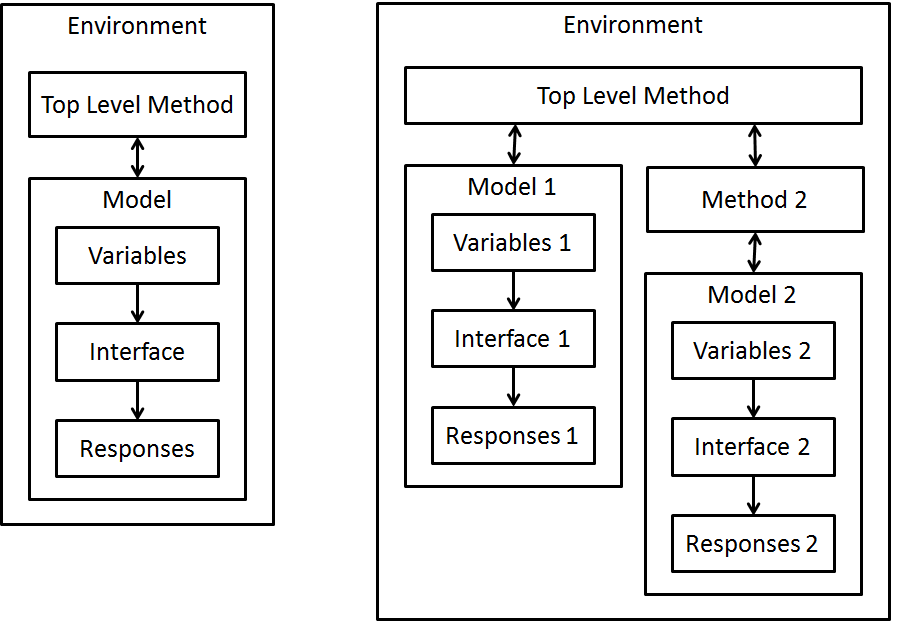
\includegraphics[height=2.5in]{images/inputfile_block_layout}
  \caption{Relationship between the six blocks, for a simple study (left)
            and an advanced, multi-method study (right)}
  \label{tutorial:inputfile_block_layout}
\end{figure}

For a more concrete example, a simple Dakota
input file, \texttt{rosen\_multidim.in}, is shown in
Figure~\ref{tutorial:rosenbrock_multidim} for a two-dimensional parameter
study on Rosenbrock's function.  This input file will be used to describe
the basic format and syntax used in all Dakota input files.  The results
are shown later, in Section~\ref{tutorial:examples:param_study}.

\begin{figure}[ht!]
  \centering
  \begin{bigbox}
    \begin{small}
      \verbatimtabinput[8]{rosen_multidim.in}
    \end{small}
  \end{bigbox}
  \caption{Rosenbrock 2-D parameter study example: the Dakota input
    file.}
  \label{tutorial:rosenbrock_multidim}
\end{figure}

Additional syntax features for Dakota input files include use of the \#
symbol to indicate a comment, use of single or double quotes for string inputs
(e.g., \texttt{'x1'}), use of commas and/or white space for separation of
specifications, and optional use of ``='' symbols to indicate
supplied data. See the Dakota Reference
Manual~\cite{RefMan} for additional details on this input file syntax.

The first block of the input file shown in
Figure~\ref{tutorial:rosenbrock_multidim} is the \emph{environment} block.
This keyword block is used to specify the general Dakota settings
such as Dakota's graphical output (via the \texttt{graphics}
flag) and the tabular data output (via the
\texttt{tabular\_graphics\_data} keyword). In addition, it 
identifies the \texttt{top\_level\_method} that will control the Dakota study.

The \emph{method} block of the input file specifies which iterative
method Dakota will employ, such as a parameter study,
optimization method, data sampling technique, etc.
The keyword \texttt{multidim\_parameter\_study}
in Figure~\ref{tutorial:rosenbrock_multidim} calls for a multidimensional
parameter study, while the keyword \texttt{partitions} specifies the
number of intervals per variable. In this case, there will be eight
intervals (nine data points) evaluated between the lower and upper
bounds of both variables (bounds provided subsequently in the
\emph{variables} section), for a total of 81 response function
evaluations.

The \emph{model} block of the input file specifies the model that
Dakota will use. A model provides the logical unit for determining
how a set of variables is mapped into a set of responses in support of
an iterative method. The model allows one to specify a single
interface, or to manage more sophisticated mappings involving
surrogates or nested iteration. For example, one might want to use
an approximate model for optimization or uncertainty quantification,
due to the lower computational cost. The
\texttt{model} keyword allows one to specify if the iterator will be
operating on a data fit surrogate (such as a polynomial regression,
neural net, etc.), a hierarchical surrogate (which uses the corrected
results of a lower fidelity simulation model as an approximation to a
higher fidelity simulation), or a nested model. See
Chapter~\ref{models} for additional model specification details. If
these advanced facilities for surrogate modeling or nested iteration
are not required, then it is not necessary to specify the
\texttt{model} keyword at all, since the default behavior is the use
of a ``single'' model constructed with the last set of responses,
variables, and interface specified. In
Figure~\ref{tutorial:rosenbrock_multidim}, the keyword \texttt{single}
explicitly specifies the use of a single model in the parameter study,
even though this is the default.

The \emph{variables} block of the input file specifies the
characteristics of the parameters that will be used in the problem
formulation. The variables can be continuous or discrete, and can be
classified as design variables, uncertain variables, or state
variables. See Chapter~\ref{variables} for more information on the
types of variables supported by Dakota. The \emph{variables} section
shown in Figure~\ref{tutorial:rosenbrock_multidim} specifies that there are
two continuous design variables. The sub-specifications for
continuous design variables
% use the abbreviation ``cdv'' in the input file and
provide the descriptors ``x1'' and ``x2'' as well as lower
and upper bounds for these variables. The information about the
variables is organized in column format for readability. So, both
variables $x_1$ and $x_2$ have a lower bound of -2.0 and an upper
bound of 2.0.

The \emph{interface} block of the input file specifies what approach
will be used to map variables into responses as well as details on how
Dakota will pass data to and from a simulation code.
In this example, the keyword \texttt{direct} is used to indicate the
use of a function linked directly into Dakota.
Alternatively, \texttt{fork} or \texttt{system} executions can be used
to invoke instances of a simulation code that is external to Dakota,
as explained in Section \ref{tutorial:examples:user_supply:optimization2} 
and Chapter~\ref{advint}.
The \texttt{analysis\_driver} keyword indicates the name of the test
function. With \texttt{fork} or \texttt{system}, default file names
would be used for passing data between Dakota and the simulation code.

The \emph{responses} block of the input file specifies the types
of data that the interface will return to Dakota. For the example
shown in Figure~\ref{tutorial:rosenbrock_multidim}, the assignment
\texttt{response\_functions = 1} indicates that there is only one response
function. Since there are no constraints associated with Rosenbrock's
function, the keywords for constraint specifications are omitted. The
keywords \texttt{no\_gradients} and \texttt{no\_hessians} indicate that
no derivatives will be provided to the method; none are needed for a
parameter study.

\section{Examples}\label{tutorial:examples}

This section serves to familiarize users with how to perform parameter 
studies, optimization, and uncertainty quantification through their common
Dakota interface. The initial examples utilize simple built in driver 
functions; later we show how to utilize Dakota to drive the evaluation of 
user supplied black box code. The examples presented in this chapter 
are intended to show the simplest use of Dakota for methods of 
each type. More advanced examples of using Dakota for specific purposes 
are provided in subsequent, topic-based, chapters.

\subsection{Rosenbrock Test Problem}\label{tutorial:examples:rosenbrock}

The examples shown later in this chapter use the Rosenbrock
function \cite{Rosenbrock60} (also described in \cite{Gil81}, among
other places), which has the form:

\begin{equation}
f(x_1,x_2)=100(x_2-x_1^2)^2+(1-x_1)^2 \label{tutorial:rosen}
\end{equation}

A three-dimensional plot of this function is shown in
Figure~\ref{tutorial:rosenbrock_prob}(a), where both $x_1$ and
$x_2$ range in value from $-2$ to $2$.
Figure~\ref{tutorial:rosenbrock_prob}(b) shows a contour plot
for Rosenbrock's function. An optimization problem using Rosenbrock's
function is formulated as follows:

\begin{eqnarray}
\texttt{minimize }   & & f(x_1,x_2)          \nonumber\\
                     & & \mathbf{x} \in \Re^2\nonumber\\
\texttt{subject to } & & -2 \le x_1 \le 2    \\
                     & & -2 \le x_2 \le 2    \nonumber
\end{eqnarray}

\begin{figure}[htp!]
  \centering
  \begin{tabular}{cc}
  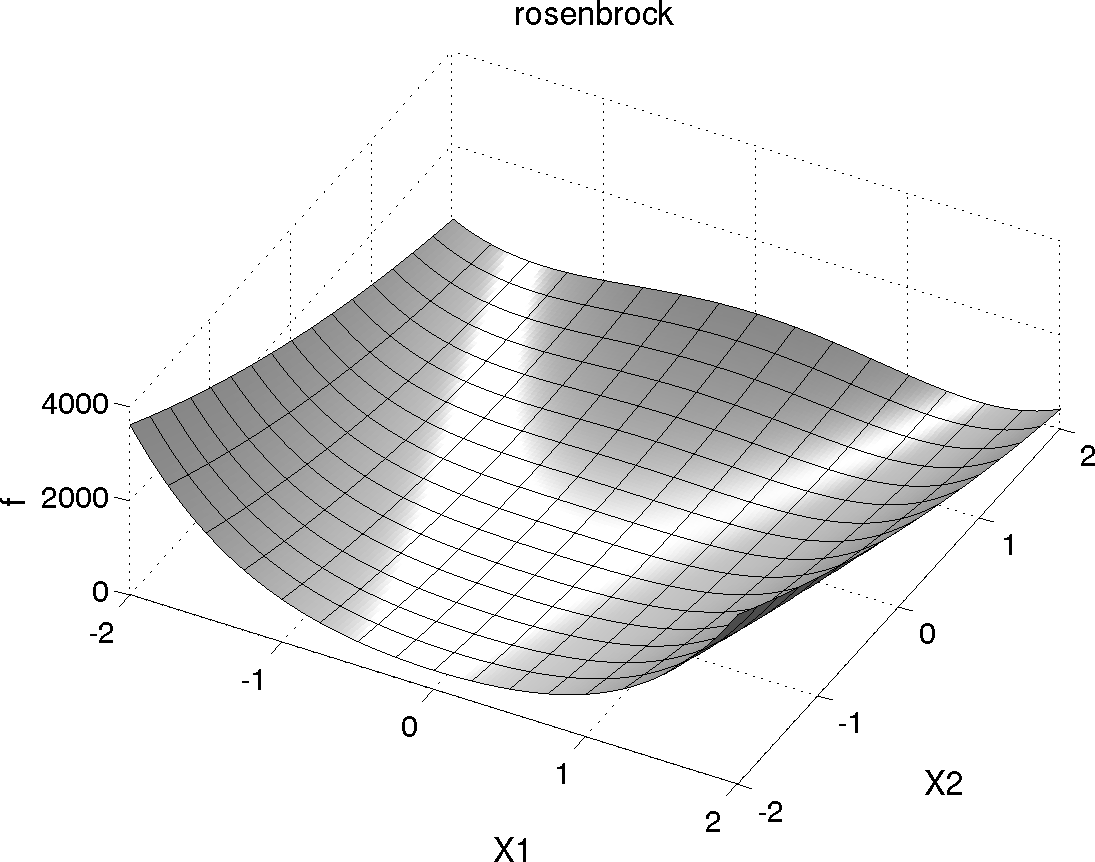
\includegraphics[height=2.5in]{images/rosen_3d_surf} &
  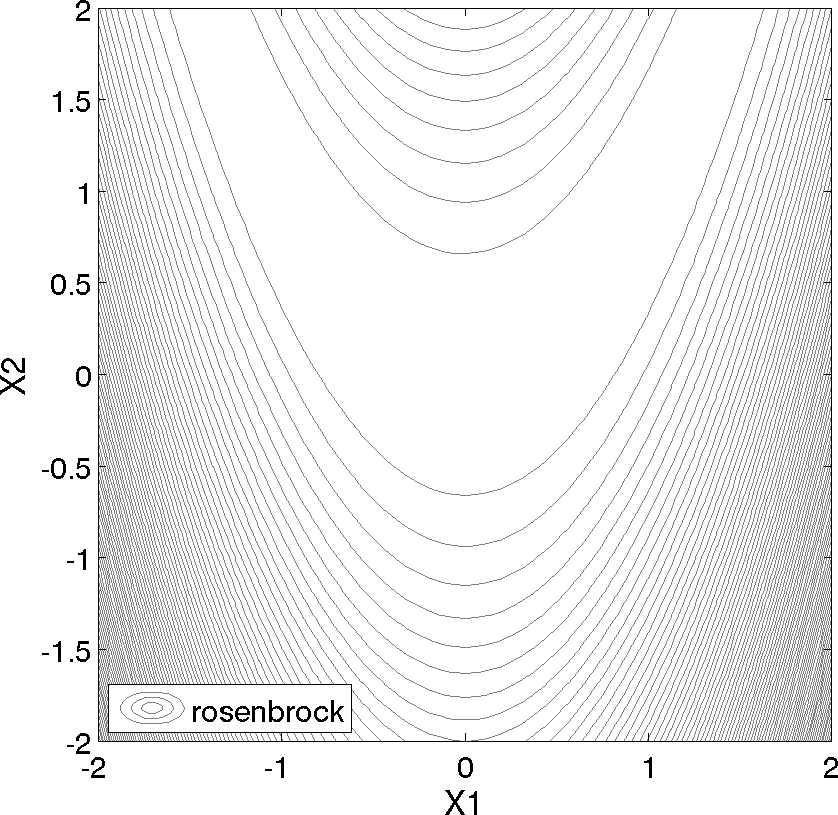
\includegraphics[height=2.5in]{images/rosen_2d_surf} \\
  (a) & (b) \\
  \end{tabular}
  \caption{Rosenbrock's function: (a) 3-D plot and (b) contours with
  $x_1$ on the bottom axis.}
  \label{tutorial:rosenbrock_prob}
\end{figure}

Note that there are no linear or nonlinear constraints in this
formulation, so this is a bound constrained optimization problem. The
unique solution to this problem lies at the point
$(x_1,x_2) = (1,1)$, where the function value is zero.

Several other test problems are available. See
Chapter~\ref{additional} for a description of these test problems
as well as further discussion of the Rosenbrock test problem.


\subsection{Two-Dimensional Grid Parameter Study}\label{tutorial:examples:param_study}

Parameter study methods in the Dakota toolkit involve the computation 
of response data sets at a selection of points in the parameter space. 
These response data sets are not linked to any specific interpretation,
so they may consist of any allowable specification from the responses 
keyword block, i.e., objective and constraint functions, least squares 
terms and constraints, or generic response functions. This allows the 
use of parameter studies in direct coordination with optimization, least 
squares, and uncertainty quantification studies without significant
modification to the input file. 

An example of a parameter study is the 2-D parameter study example problem 
listed in Figure~\ref{tutorial:rosenbrock_multidim}. This is 
executed by Dakota using the command noted in the comments:
\begin{small}
\begin{verbatim}
    dakota -i rosen_multidim.in -o rosen_multidim.out > rosen_multidim.stdout
\end{verbatim}
\end{small}

The output of the Dakota run is written to the file named
\texttt{rosen\_multidim.out} while the screen output, or
standard output, is redirect to \texttt{rosen\_multidim.stdout}.
For comparison, files named \texttt{rosen\_multidim.out.sav}
and \texttt{rosen\_multidim.stdout.sav} are included in the
\texttt{Dakota/examples/users} directory. As for many of the examples,
Dakota provides a report on the best design point located during the
study at the end of these output files.

This 2-D parameter study produces the grid of data samples shown in
Figure~\ref{tutorial:rosenbrock_multidim_graphics}. In general, a multidimensional 
parameter study lets one generate a grid in multiple dimensions. 
The keyword \texttt{multidim\_parameter\_study} indicates that 
a grid will be generated over all variables. The keyword 
\texttt{partitions} indicates the number of grid partitions in 
each dimension. For this example, the number of the grid partitions 
are the same in each dimension (8 partitions) but it would be possible 
to specify (partitions = 8 2), and have only two partitions 
over the second input variable.  Note that the
\texttt{graphics} flag in the \emph{environment} block of the input
file could be commented out since, for this example, the iteration
history plots created by Dakota are not particularly instructive. More
interesting visualizations can be created by importing Dakota's
tabular data into an external graphics/plotting package. Common
graphics and plotting packages include Mathematica, Matlab, Microsoft
Excel, Origin, Tecplot, Gnuplot and many others. (Sandia National Laboratories
and the Dakota developers do not endorse any of these commercial
products.)

\begin{figure}[htb!]
  \centering
  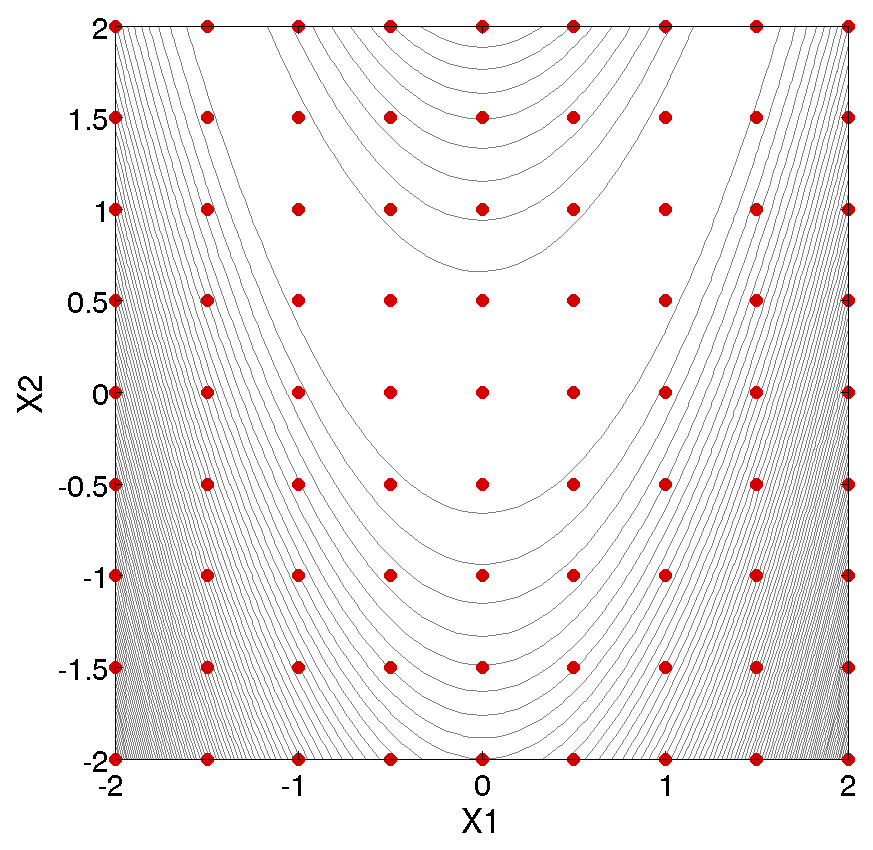
\includegraphics[height=2.5in]{images/rosen_2d_pts}
  \caption{Rosenbrock 2-D parameter study example:
  location of the design points (dots) evaluated.}
  \label{tutorial:rosenbrock_multidim_graphics}
\end{figure}


\subsection{Gradient-based Unconstrained Optimization}\label{tutorial:examples:optimization}

Dakota's optimization capabilities include a variety of gradient-based 
and nongradient-based optimization methods. This subsection demonstrates
the use of one such method through the Dakota interface.

A Dakota input file for a gradient-based optimization of Rosenbrock's
function is listed in Figure~\ref{tutorial:rosenbrock_grad}. The
format of the input file is similar to that used for the parameter
studies, but there are some new keywords in the responses and method
sections. First, in the responses block of the input file, the
keyword block starting with \texttt{numerical\_gradients} specifies
that a finite difference method will be used to compute gradients for
the optimization algorithm. Note that the Rosenbrock function
evaluation code inside Dakota has the ability to give analytical
gradient values. (To switch from finite difference gradient estimates
to analytic gradients, uncomment the \texttt{analytic\_gradients}
keyword and comment out the four lines associated with the
\texttt{numerical\_gradients} specification.)
Next, in the method
block of the input file, several new keywords have been added. In
this block, the keyword \texttt{conmin\_frcg} indicates the use of
the Fletcher-Reeves conjugate gradient algorithm in the CONMIN
optimization software package~\cite{Van78} for bound-constrained
optimization. The keyword \texttt{max\_iterations} is used to
indicate the computational budget for this optimization (in this case,
a single iteration includes multiple evaluations of Rosenbrock's
function for the gradient computation steps and the line search
steps). The keyword \texttt{convergence\_tolerance} is used to specify
one of CONMIN's convergence criteria (under which CONMIN terminates if the
objective function value differs by less than the absolute value of
the convergence tolerance for three successive iterations).
% And, finally, the \texttt{output} verbosity is set to \texttt{quiet}.

\begin{figure}
  \centering
  \begin{bigbox}
    \begin{small}
      \verbatimtabinput[8]{rosen_grad_opt.in}
    \end{small}
  \end{bigbox}
  \caption{Rosenbrock gradient-based unconstrained optimization
  example: the Dakota input file.}
  \label{tutorial:rosenbrock_grad}
\end{figure}

The Dakota command is noted in the file, and copies of the outputs
are in the \texttt{Dakota/examples/users} directory, with \texttt{.sav}
appended to the name.  When this example problem is executed using
Dakota with graphics support enabled, Dakota creates some iteration
history graphics similar to the screen capture shown in Figure~
\ref{tutorial:rosenbrock_grad_graphics}(a). These plots show how the
objective function and design parameters change in value during the
optimization steps. The scaling of the horizontal and vertical axes
can be changed by moving the scroll knobs on each plot.  Also, the
``Options'' button allows the user to plot the vertical axes using a
logarithmic scale. Note that log-scaling is only allowed if the values
on the vertical axis are strictly greater than zero.

\begin{figure}[ht!]
  \centering
  \begin{tabular}{c}
  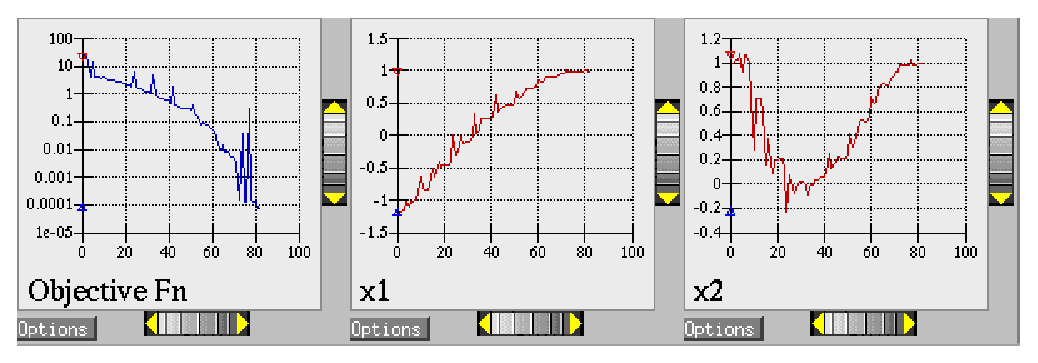
\includegraphics[width=\textwidth]{images/dak_graphics_grad_opt}\\
  (a)\\
  \qquad\\
  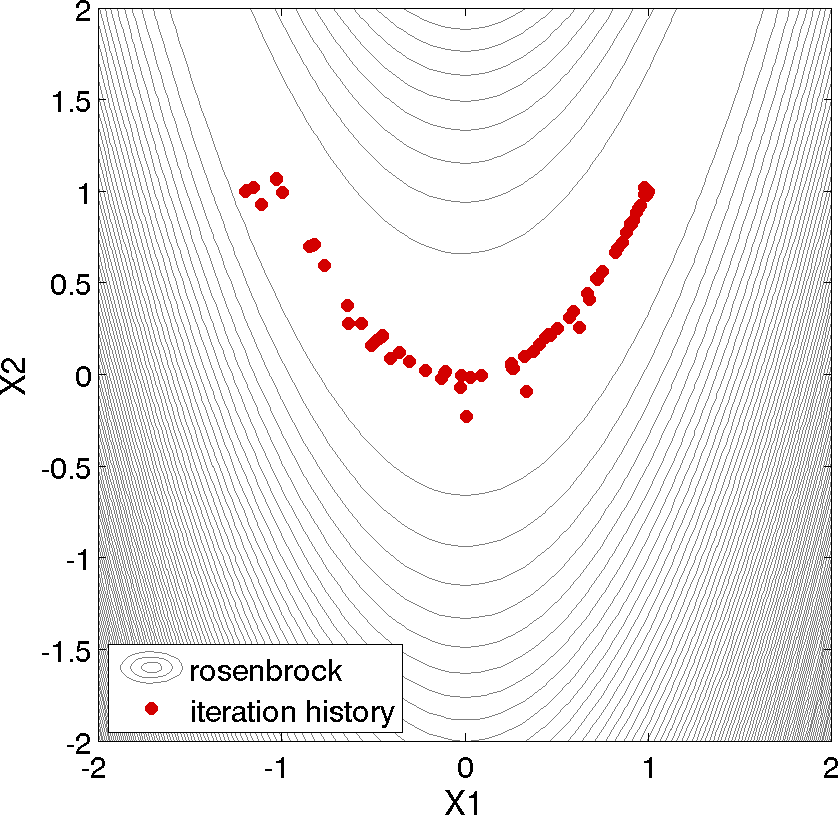
\includegraphics[height=2.5in]{images/rosen_grad_opt_pts} \\
  (b)
  \end{tabular}
  \caption{Rosenbrock gradient-based unconstrained optimization
    example: (a) screen capture of the Dakota graphics and (b)
    sequence of design points (dots) evaluated (line search points
    omitted).}
  \label{tutorial:rosenbrock_grad_graphics}
\end{figure}

Figure~\ref{tutorial:rosenbrock_grad_graphics}(b) shows the
iteration history of the optimization algorithm. The optimization
starts at the point $(x_1,x_2) = (-1.2,1.0)$ as given in the
Dakota input file. Subsequent iterations follow the banana-shaped
valley that curves around toward the minimum point at $(x_1,x_2) =
(1.0,1.0)$. Note that the function evaluations associated with the
line search phase of each CONMIN iteration are not shown on the plot.
At the end of the Dakota run, information is written to the output
file to provide data on the optimal design point. These data include
the optimum design point parameter values, the optimum objective and
constraint function values (if any), plus the number of function
evaluations that occurred and the amount of time that elapsed during
the optimization study.

\subsection{Uncertainty Quantification with Monte Carlo Sampling}\label{tutorial:examples:uncert_quant}

Uncertainty quantification (UQ) is the process of determining the
effect of input uncertainties on response metrics of interest. These
input uncertainties may be characterized as either aleatory
uncertainties, which are irreducible variabilities inherent in nature,
or epistemic uncertainties, which are reducible uncertainties
resulting from a lack of knowledge. Since sufficient data is
generally available for aleatory uncertainties, probabilistic methods
are commonly used for computing response distribution statistics based
on input probability distribution specifications. Conversely, for
epistemic uncertainties, data is generally sparse, making the use of
probability theory questionable and leading to nonprobabilistic
methods based on interval specifications.

The subsection demonstrates the use of Monte Carlo random sampling
for Uncertainty Quantification.

Figure~\ref{tutorial:rosenbrock_mc} shows the Dakota input file for
an example problem that demonstrates some of the random sampling
capabilities available in Dakota. In this example, the design
parameters, x1 and x2, will be treated as uncertain parameters that
have uniform distributions over the interval [-2, 2]. This is
specified in the variables block of the input file, beginning with
the keyword \texttt{uniform\_uncertain}.
% Not true: For comparison, the keywords
% from the previous examples are retained, but have been commented out.
Another difference from earlier input files such as
Figure~\ref{tutorial:rosenbrock_grad}
occurs in the responses block, where
the keyword \texttt{response\_functions} is used in place of
\texttt{objective\_functions}. The final changes to the input
file occur in the method block, where the keyword
\texttt{sampling} is used.

The other keywords in the methods block of the input file
specify the number of samples (200), the seed for the random number
generator (17), the sampling method (random), and the response
threshold (100.0). The \texttt{seed} specification allows a user to
obtain repeatable results from multiple runs. If a seed value is not
specified, then Dakota's sampling methods are designed to generate
nonrepeatable behavior (by initializing the seed using a system
clock). The keyword \texttt{response\_levels} allows the user to
specify threshold values for which Dakota will compute statistics on
the response function output. Note that a unique threshold value can
be specified for each response function.

In this example, Dakota will select 200 design points from within the
parameter space, evaluate the value of Rosenbrock's function at all
200 points, and then perform some basic statistical calculations on
the 200 response values.

The Dakota command is noted in the file, and copies of the outputs
are in the \texttt{Dakota/examples/users} directory, with \texttt{.sav} 
appended to the name.  
Figure~\ref{tutorial:results_mc} shows example results from this 
sampling method. 
Note that your results will differ from those in
this file if your \texttt{seed} value differs or if no \texttt{seed}
is specified.

As shown in Figure~\ref{tutorial:results_mc}, 
the statistical data on the 200 Monte Carlo samples is printed at the
end of the output file in the section that starts with ``Statistics
based on 200 samples.'' In this section summarizing 
moment-based statistics, Dakota outputs the
mean, standard deviation, skewness, and kurtosis estimates 
for each of the response functions. For example, 
the mean of the Rosenbrock function given uniform input uncertainties 
on the input variables is 455.4 and the standard deviation is 536.8. 
This is a very large standard deviation, due to the fact that the 
Rosenbrock function varies by three orders of magnitude over the input 
domain. The skewness is positive, meaning this is a right-tailed distribution, 
not a symmetric distribution. Finally, the kurtosis (a measure of the 
``peakedness'' of the distribution) indicates that 
this is a strongly peaked distribution (note that we use a central, 
standardized kurtosis so that the kurtosis of a normal is zero). 
After the moment-related statistics, the 95\% confidence intervals on the 
mean and standard deviations are printed. This is followed by
the fractions (``Probability Level'') of the response function values 
that are below the response threshold values specified in the input file. 
For example, 34 percent of the sample inputs resulted in a Rosenbrock 
function value that was less than or equal to 100, as shown in the line 
listing the cumulative distribution function values. 
Finally, there are several 
correlation matrices printed at the end, showing simple and partial 
raw and rank correlation matrices. Correlations provide an indication 
of the strength of a monotonic relationship between input and outputs. 
More detail on correlation coefficients and their interpretation can be 
found in Section~\ref{uq:uncertainty1}. 
More detail about sampling methods in general can be found in 
Section~\ref{uq:sampling}. Finally,  
Figure~\ref{tutorial:rosenbrock_mc_points} shows the locations
of the 200 sample sites within the parameter space of the Rosenbrock
function for this example.

\begin{figure}[ht!]
  \centering
  \begin{bigbox}
    \begin{small}
      \verbatimtabinput[8]{rosen_sampling.in}
    \end{small}
  \end{bigbox}
  \caption{Monte Carlo sampling example: the Dakota input file.}
  \label{tutorial:rosenbrock_mc}
\end{figure}

\begin{figure}
\centering
\begin{bigbox}
\begin{footnotesize}
\begin{verbatim}
Statistics based on 200 samples:

Moment-based statistics for each response function:
                            Mean           Std Dev          Skewness          Kurtosis
 response_fn_1  4.5540183516e+02  5.3682678089e+02  1.6661798252e+00  2.7925726822e+00

95% confidence intervals for each response function:
                    LowerCI_Mean      UpperCI_Mean    LowerCI_StdDev    UpperCI_StdDev
 response_fn_1  3.8054757609e+02  5.3025609422e+02  4.8886795789e+02  5.9530059589e+02

Level mappings for each response function:
Cumulative Distribution Function (CDF) for response_fn_1:
     Response Level  Probability Level  Reliability Index  General Rel Index
     --------------  -----------------  -----------------  -----------------
   1.0000000000e+02   3.4000000000e-01

Probability Density Function (PDF) histograms for each response function:
PDF for response_fn_1:
          Bin Lower          Bin Upper      Density Value
          ---------          ---------      -------------
   1.1623549854e-01   1.0000000000e+02   3.4039566059e-03
   1.0000000000e+02   2.7101710856e+03   2.5285698843e-04

Simple Correlation Matrix among all inputs and outputs:
                       x1           x2 response_fn_1 
          x1  1.00000e+00 
          x2 -5.85097e-03  1.00000e+00 
response_fn_1 -9.57746e-02 -5.08193e-01  1.00000e+00 

Partial Correlation Matrix between input and output:
             response_fn_1 
          x1 -1.14659e-01 
          x2 -5.11111e-01 

Simple Rank Correlation Matrix among all inputs and outputs:
                       x1           x2 response_fn_1 
          x1  1.00000e+00 
          x2 -6.03315e-03  1.00000e+00 
response_fn_1 -1.15360e-01 -5.04661e-01  1.00000e+00 

Partial Rank Correlation Matrix between input and output:
             response_fn_1 
          x1 -1.37154e-01 
          x2 -5.08762e-01 
\end{verbatim}
\end{footnotesize}
\end{bigbox}
\caption{Results of Monte Carlo Sampling on the Rosenbrock Function}
\label{tutorial:results_mc}
\end{figure}


\begin{figure}[ht!]
  \centering
  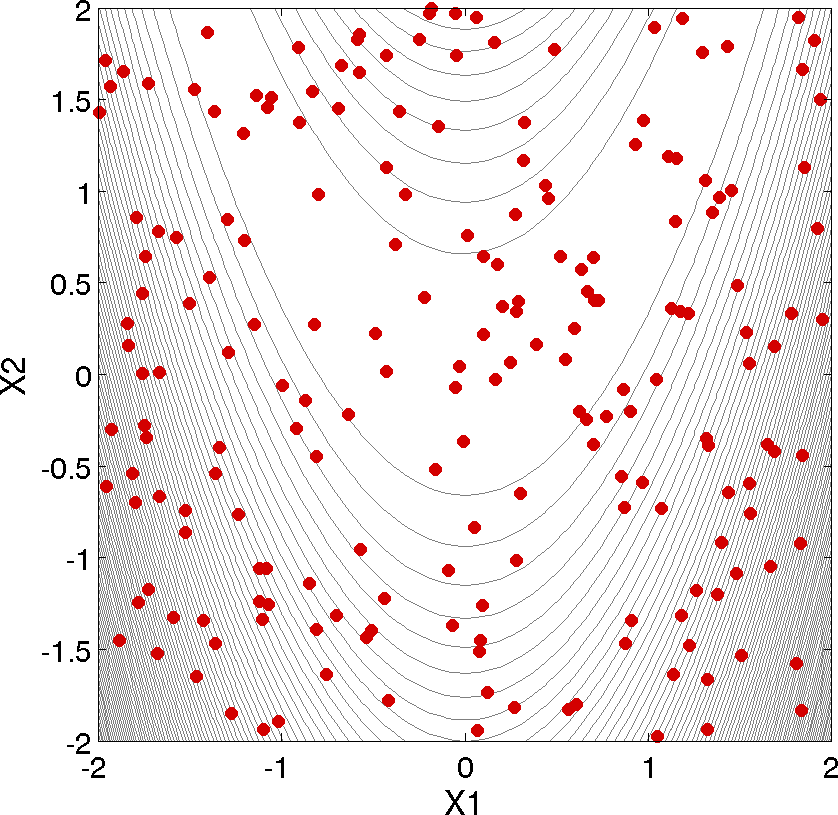
\includegraphics[height=2.5in]{images/rosen_nond_pts}
  \caption{Monte Carlo sampling example: locations in the parameter
    space of the 200 Monte Carlo samples using a uniform distribution
    for both $x_1$ and $x_2$.}
  \label{tutorial:rosenbrock_mc_points}
\end{figure}

\subsection{User Supplied Simulation Code Examples}\label{tutorial:examples:user_supply}
This subsection provides examples of how to use Dakota to drive user 
supplied black box code.

\subsubsection{Optimization with a User-Supplied Simulation Code - Case 1}\label{tutorial:examples:user_supply:optimization1}

Many of the previous examples made use of the direct interface to
access the Rosenbrock and textbook test functions that are compiled
into Dakota. In engineering applications, it is much more common to
use the \texttt{fork} interface approach within
Dakota to manage external simulation codes. In both of these cases,
the communication between Dakota and the external code is conducted
through the reading and writing of short text files. For this example,
the C++ program \texttt{rosenbrock.cpp} in \texttt{Dakota\_Source/test} is used
as the simulation code. This file is compiled to create the
stand-alone \texttt{rosenbrock} executable that is referenced as the
\texttt{analysis\_driver} in Figure~\ref{tutorial:rosenbrock_user}.
This stand-alone program performs the same function evaluations as
Dakota's internal Rosenbrock test function.

Figure~\ref{tutorial:rosenbrock_user} shows the text of the Dakota
input file named \texttt{rosen\_syscall.in} that is
provided in the directory \texttt{Dakota/examples/users}.
The only differences between this input file and the one in Figure~
\ref{tutorial:rosenbrock_grad} occur in the \emph{interface} keyword
section. The keyword \texttt{fork} indicates that Dakota will use
fork calls to create separate Unix processes for executions of the
user-supplied simulation code. The name of the simulation code, and
the names for Dakota's parameters and results file are specified using
the \texttt{analysis\_driver}, \texttt{parameters\_file}, and
\texttt{results\_file} keywords, respectively.

The Dakota command is noted in the file, and copies of the outputs
are in the \texttt{Dakota/examples/users} directory, with \texttt{.sav} 
appended to the name.  

This run of Dakota takes longer to complete than the previous
gradient-based optimization example since the \texttt{fork}
interface method has additional process creation and file I/O
overhead, as compared to the internal communication that occurs when
the \texttt{direct} interface method is used. 

To gain a better understanding of what exactly Dakota is doing with
the \texttt{fork} interface approach, add the keywords
\texttt{file\_tag} and \texttt{file\_save} to the interface
specification and re-run Dakota. Check the listing of the local
directory and you will see many new files with names such as
\texttt{params.in.1}, \texttt{params.in.2}, etc., and
\texttt{results.out.1}, \texttt{results.out.2}, etc. There is one
\texttt{params.in.X} file and one \texttt{results.out.X} file for each
of the function evaluations performed by Dakota. This is the file
listing for \texttt{params.in.1}:
%\newpage
\begin{small}
\begin{verbatim}
                                          2 variables
                     -1.200000000000000e+00 x1
                      1.000000000000000e+00 x2
                                          1 functions
                                          1 ASV_1:obj_fn
                                          2 derivative_variables
                                          1 DVV_1:x1
                                          2 DVV_2:x2
                                          0 analysis_components
\end{verbatim}
\end{small}

\begin{figure}[b!]
  \begin{bigbox}
    \begin{small}
      \verbatimtabinput[8]{rosen_syscall.in}
    \end{small}
  \end{bigbox}
  \caption{Dakota input file for gradient-based optimization using the
    fork call interface to an external rosenbrock simulator.}
  \label{tutorial:rosenbrock_user}
\end{figure}

The basic pattern is that of array lengths and string identifiers
followed by listings of the array entries, where the arrays consist of
the variables, the active set vector (ASV), the derivative values
vector (DVV), and the analysis components (AC). For the variables
array, the first line gives the total number of variables (2) and the
``variables'' string identifier, and the subsequent two lines provide
the array listing for the two variable values (-1.2 and 1.0) and
descriptor tags (``x1'' and ``x2'' from the Dakota input file). The
next array conveys the ASV, which indicates what
simulator outputs are needed. The first line of the array gives the total number
of response functions (1) and the ``functions'' string identifier,
followed by one ASV code and descriptor tag
(``ASV\_1'') for each function. In this case, the ASV value of 1 indicates that Dakota
is requesting that the simulation code return the response function
value in the file \texttt{results.out.X}. (Possible ASV values: 1 = value of
response function value, 2 = response function gradient, 4 = response
function Hessian, and any sum of these for combinations up to
7 = response function value, gradient, and Hessian; see ~\ref{variables:asv} for
more detail.)  The next array provides the DVV, which defines the
variable identifiers used in computing derivatives. The first line of
the array gives the number of derivative variables (2) and the
``derivative\_variables'' string identifier, followed by the listing of
the two DVV variable identifiers (the first and second variables) and
descriptor tags (``DVV\_1'' and ``DVV\_2''). The final array provides
the AC array used to provide additional strings for use by the
simulator (e.g., to provide the name of a particular mesh file). The
first line of the array gives the total number of analysis components
(0) and the ``analysis\_components'' string identifier, followed by the
listing of the array, which is empty in this case.

The executable program rosenbrock reads in the \texttt{params.in.X}
file and evaluates the objective function at the given values for
$x_1$ and $x_2$. Then, rosenbrock writes out
the objective function data to the \texttt{results.out.X} file. Here
is the listing for the file \texttt{results.out.1}:
\begin{small}
\begin{verbatim}
                     2.420000000000000e+01 f
\end{verbatim}
\end{small}

The value shown above is the value of the objective function, and the
descriptor `f' is an optional tag returned by the simulation code.
When the fork call has completed, Dakota reads in the data from the
\texttt{results.in.X} file and processes the results. Dakota then
continues with additional executions of the rosenbrock program until
the optimization process is complete.

\subsubsection{Optimization with a User-Supplied Simulation Code - Case 2}\label{tutorial:examples:user_supply:optimization2}

In many situations the user-supplied simulation code cannot be
modified to read and write the \texttt{params.in.X file} and the
\texttt{results.out.X} file, as described above. Typically, this
occurs when the simulation code is a commercial or proprietary
software product that has specific input file and output file formats.
In such cases, it is common to replace the executable program name in
the Dakota input file with the name of a Unix shell script containing
a sequence of commands that read and write the necessary files and run
the simulation code. For example, the executable program named
\texttt{rosenbrock} listed in Figure~\ref{tutorial:rosenbrock_user}
could be replaced by a Unix Bourne or C-shell script named
\texttt{simulator\_script}, with the script containing a sequence of
commands to perform the following steps: insert the data from the
\texttt{parameters.in.X} file into the input file of the simulation
code, execute the simulation code, post-process the files generated by
the simulation code to compute response data, and return the response
data to Dakota in the \texttt{results.out.X} file. The steps that are
typically used in constructing and using a Unix shell script are
described in Section~\ref{interfaces:building}.

\section{Dakota Command-Line Options}\label{tutorial:installation:running}

The Dakota executable file is named {\tt dakota} ({\tt dakota.exe} on
Windows). If this command is entered at the command prompt without any
arguments, a usage message similar to the following appears:
\begin{small}
\begin{verbatim}
usage: dakota [options and <args>]
        -help (Print this summary)
        -version (Print Dakota version number)
        -input <$val> (REQUIRED Dakota input file $val)
        -output <$val> (Redirect Dakota standard output to file $val)
        -error <$val> (Redirect Dakota standard error to file $val)
        -parser <$val> (Parsing technology: nidr[strict][:dumpfile])
        -no_input_echo (Do not echo Dakota input file)
        -check (Perform input checks)
        -pre_run [$val] (Perform pre-run (variables generation) phase)
        -run [$val] (Perform run (model evaluation) phase)
        -post_run [$val] (Perform post-run (final results) phase)
        -read_restart [$val] (Read an existing Dakota restart file $val)
        -stop_restart <$val> (Stop restart file processing at evaluation $val)
        -write_restart [$val] (Write a new Dakota restart file $val)
\end{verbatim}
\end{small}
%$ this comment is here to trick xemacs into highlighting syntax correctly

Of these available command line inputs, only the ``\texttt{-input}''
option is required, and ``\texttt{-input}'' can be omitted if the
input file name is the final item on the command line; all other
command-line inputs are optional. The ``\texttt{-help}'' option prints
the usage message above. The ``\texttt{-version}'' option prints the
version number of the executable. The ``\texttt{-check}'' option
invokes a dry-run mode in which the input file is processed and
checked for errors, but the study is not performed. The
``\texttt{-input}'' option provides the name of the Dakota input file.
The ``\texttt{-output}'' and ``\texttt{-error}'' options provide file
names for redirection of the Dakota standard output (stdout) and
standard error (stderr), respectively. By default, Dakota will echo
the input file to the output stream, but ``\texttt{-no\_input\_echo}''
can override this behavior.

The ``\texttt{-parser}'' input is for debugging and will not
be further described here. The ``\texttt{-read\_restart}''
and ``\texttt{-write\_restart}'' options provide the names of
restart databases to read from and write to, respectively. The
``\texttt{-stop\_restart}'' option limits the number of
function evaluations read from the restart database (the default is all
the evaluations) for those cases in which some evaluations were erroneous
or corrupted. Restart management is an important technique for retaining
data from expensive engineering applications. This advanced topic is
discussed in detail in Chapter~\ref{restart}. Note that these command
line options can be abbreviated so long as the abbreviation is unique.
Accordingly, the following are valid, unambiguous specifications: ``\texttt{-h}'',
``\texttt{-v}'', ``\texttt{-c}'', ``\texttt{-i}'', ``\texttt{-o}'',
``\texttt{-e}'', ``\texttt{-re}'', ``\texttt{-s}'', ``\texttt{-w}'',
``\texttt{-pr}'', ``\texttt{-ru}'', and ``\texttt{-po}'' and can be used
in place of the longer forms of the command line options.

To run Dakota with a particular input file, the following syntax can
be used:
\begin{small}
\begin{verbatim}
    dakota -i dakota.in
\end{verbatim}
\end{small}
or more simply
\begin{small}
\begin{verbatim}
    dakota dakota.in
\end{verbatim}
\end{small}

This will echo the standard output (stdout) and standard error
(stderr) messages to the terminal. To redirect stdout and stderr to
separate files, the \texttt{-o} and \texttt{-e} command line options
may be used:
\begin{small}
\begin{verbatim}
    dakota -i dakota.in -o dakota.out -e dakota.err
\end{verbatim}
\end{small}
or
\begin{small}
\begin{verbatim}
    dakota -o dakota.out -e dakota.err dakota.in
\end{verbatim}
\end{small}

Alternatively, any of a variety of Unix redirection variants can be
used. The simplest of these redirects stdout to another file:
\begin{small}
\begin{verbatim}
    dakota dakota.in > dakota.out
\end{verbatim}
\end{small}

% this is not a linux tutorial.
% To append to a file rather than overwrite it, ``\texttt{>>}'' is used
% in place of ``\texttt{>}''. The syntax to redirect stderr as well as stdout
% to the same file depends on the shell you are using. With csh, simply append
% ``\texttt{\&}'' with no embedded space, i.e.,
% ``\texttt{>\&}'' or ``\texttt{>>\&}''. With the Bourne shell (sh or bash) use
% ``\texttt{>dakota.out 2>\&1}'' or ``\texttt{>>dakota.out 2>\&1}''.
% With csh, if you have the noclobber environment variable set but
% wish either to overwrite an existing output file or to append to a file that
% does not yet exist, append ``\texttt{!}'' to the redirection operators
% (with no intervening spaces), i.e.,
% ``\texttt{>!}'', ``\texttt{>\&!}'', ``\texttt{>>!}'', or
% ``\texttt{>>\&!}''.

To run the dakota process in the background, append an ampersand
symbol (\&) to the command with an embedded space, e.g.,
\begin{small}
\begin{verbatim}
    dakota dakota.in > dakota.out &
\end{verbatim}
\end{small}

Refer to~\cite{And86} for more information on Unix redirection and
background commands.

The ``\texttt{-pre\_run}'', ``\texttt{-run}'', and
``\texttt{-post\_run}'' options instruct Dakota to run one or more
execution phases, excluding others. For example pre-run might
generate variable sets, run (core run) might invoke the simulation to
evaluate variables and produce responses, and post-run might accept
variable/response sets and analyzes the results (for example,
calculate correlations from a set of samples). Currently only two
modes are supported and only for sampling, parameter study, and DACE
methods: (1) pre-run only with optional tabular output of variables:
\begin{small}
\begin{verbatim}
    dakota -i dakota.in -pre_run [::myvariables.dat]
\end{verbatim}
\end{small}
and (2) post-run only with required tabular input of variables/responses:
\begin{small}
\begin{verbatim}
    dakota -i dakota.in -post_run myvarsresponses.dat::
\end{verbatim}
\end{small}


\section{Next Steps}\label{tutorial:nextsteps}

After reading this chapter, you should understand the mechanics of
acquiring, installing, and executing Dakota to perform simple studies.
You should have a high-level appreciation for what inputs Dakota
requires, how it behaves during interfacing and operation for a few
kinds of studies, and what representative output is obtained.  To
effectively use Dakota, you will need to understand the character of
your problem, select a Dakota method to help you meet your analysis
goals, and develop an interface to your computational model.

\subsection{Problem Exploration and Method Selection}\label{tutorial:exploration}

Section~\ref{intro:capabilities} provides a high-level overview of the
analysis techniques available in Dakota, with references to more
details and usage guidelines in the following chapters.  Selecting an
appropriate method to meet your analysis goals requires understanding
problem characteristics.  For example, in optimization, typical
questions that should be addressed include: Are the design variables
continuous, discrete, or mixed? Is the problem constrained or
unconstrained? How expensive are the response functions to evaluate?
Will the response functions behave smoothly as the design variables
change or will there be nonsmoothness and/or discontinuities? Are the
response functions likely to be multimodal, such that global
optimization may be warranted? Is analytic gradient data available,
and if not, can gradients be calculated accurately and cheaply?
Questions pertinent for uncertainty quantification may include: Can I
accurately model the probabilistic distributions of my uncertain
variables? Are the response functions relatively linear? Am I
interested in a full random process characterization of the response
functions, or just statistical results?

If there is not sufficient information from the problem description
and prior knowledge to answer these questions, then additional problem
characterization activities may be warranted. Dakota parameter studies
and design of experiments methods can help answer these questions by
systematically interrogating the model.  The resulting trends in the
response functions can be evaluated to determine if these trends are
noisy or smooth, unimodal or multimodal, relatively linear or highly
nonlinear, etc. In addition, the parameter studies may reveal that one
or more of the parameters do not significantly affect the results and
can be omitted from the problem formulation. This can yield a
potentially large savings in computational expense for the subsequent
studies. Refer to Chapters~\ref{ps} and~\ref{dace} for additional
information on parameter studies and design of experiments methods.

For a list of all the example Dakota input files, see 
Table~\ref{tutorial:examples:table}. All of these input files 
can be found in \\ \texttt{Dakota/examples/users}. 

\begin{table}[hbp]
\centering
\caption{List of Example Input Files}
\label{tutorial:examples:table}\vspace{2mm}
\begin{tabular}{|c|c|c|c|}
\hline
\textbf{Method Category} & \textbf{Specific Method} & 
\textbf{Input File Name} & \textbf{Reference}\\
\hline
parameter study & multidimensional parameter study & rosen\_multidim.in &~\ref{tutorial:rosenbrock_multidim} \\
parameter study & vector parameter study & rosen\_ps\_vector.in & ~\ref{additional:rosenbrock_vector} \\
design of comp exp & moat (Morris) & morris\_ps\_moat.in & ~\ref{FIG:moat:out_preamble} \\
uncertainty quantification & random sampling & rosen\_sampling.in & ~\ref{tutorial:rosenbrock_mc}\\
uncertainty quantification & LHS sampling & textbook\_uq\_sampling.in & ~\ref{uq:figure01}\\
uncertainty quantification & polynomial chaos expansion & rosen\_uq\_pce.in & ~\ref{uq:examples:pce_input} \\
uncertainty quantification & stochastic collocation & rosen\_uq\_sc.in & ~\ref{uq:figure11} \\
uncertainty quantification & reliability Mean Value & textbook\_uq\_meanvalue.in & ~\ref{uq:examples:mv_input} \\
uncertainty quantification & reliability FORM & logratio\_uq\_reliability.in & ~\ref{uq:rel_input_form} \\
uncertainty quantification & global interval analysis & cantilever\_uq\_global\_interval.in & ~\ref{uq:examples:interval_input} \\
uncertainty quantification & global evidence analysis & textbook\_uq\_glob\_evidence.in & ~\ref{uq:figure16} \\
optimization & gradient-based, unconstrained & rosen\_grad\_opt.in & ~\ref{tutorial:rosenbrock_grad} \\
optimization & gradient-based, unconstrained & rosen\_syscall.in  & ~\ref{tutorial:rosenbrock_user} \\
optimization & gradient-based, constrained & textbook\_opt\_conmin.in & ~\ref{additional:textbook_grad_constr} \\
optimization & gradient-based, constrained & cantilever\_opt\_npsol.in & ~\ref{additional:cant_opt_npsol} \\
optimization & gradient-based, constrained & container\_opt\_npsol.in & ~\ref{output:incont} \\
optimization & evolutionary algorithm & rosen\_opt\_ea.in  & ~\ref{opt:methods:gradientfree:global:example:rosenbrock_ea} \\
optimization & pattern search & rosen\_opt\_patternsearch.in  & ~\ref{opt:methods:gradientfree:local:example:ps} \\
optimization & efficient global optimization (EGO) & rosen\_opt\_ego.in  & ~\ref{opt:methods:gradientfree:global:example:egm_rosen}\\
optimization & efficient global optimization (EGO) & herbie\_shubert\_opt\_ego.in  & ~\ref{additional:herbie_shubert_ego}\\
optimization & multiobjective  & textbook\_opt\_multiobj1.in  & ~\ref{opt:additional:multiobjective:example1:figure01}\\
optimization & Pareto opt., moga  & mogatest1.in  & ~\ref{opt:additional:multiobjective:example2:moga1inp}\\
optimization & Pareto opt., moga  & mogatest2.in  & ~\ref{additional:moga2inp}\\
optimization & Pareto opt., moga  & mogatest3.in  & ~\ref{additional:moga3inp}\\
optimization & optimization with scaling  & rosen\_opt\_scaled.in  & ~\ref{opt:additional:scaling:example:figure01}\\
calibration & nonlinear least squares  & rosen\_opt\_nls.in  & ~\ref{additional:rosenbrock_nls}\\
calibration & NLS with datafile  & textbook\_nls\_datafile.in  & \\
advanced methods & hybrid minimization & textbook\_hybrid\_strat.in  & ~\ref{adv_meth:figure01}\\
advanced methods & Pareto minimization & textbook\_pareto\_strat.in  & ~\ref{adv_meth:figure04}\\
advanced methods & multistart minimization & qsf\_multistart\_strat.in  & ~\ref{adv_meth:figure02}\\
advanced methods & surrogate based global & mogatest1\_opt\_sbo.in  & ~\ref{sbm:sbgm_moga}\\
advanced methods & surrogate based local  & rosen\_opt\_sbo.in  & ~\ref{sbm:sblm_rosen}\\
advanced models  & opt. under uncertainty (OUU) & textbook\_opt\_ouu1.in  & ~\ref{adv_models:figure09}\\
advanced models  & second order probability & cantilever\_uq\_sop\_rel.in & ~\ref{adv_models:2ndprob} \\
advanced models  & sampling on a surrogate model & textbook\_uq\_surrogate.in & \\
\hline
\end{tabular}
\end{table}

 
\subsection{Key Getting Started References}\label{tutorial:keyrefs}

The following references address many of the most common questions
raised by new Dakota users:
\begin{itemize}
\item Dakota documentation and training materials are available from
  the Dakota website \url{http://dakota.sandia.gov}.

\item Dakota input file syntax (valid keywords and settings) is
  described in the Dakota Reference Manual~\cite{RefMan}.

\item Example input files are included throughout this manual, and
  are included in Dakota distributions and installations. See
  Section~\ref{intro:files} for help finding these files.

\item Detailed method descriptions appear in the Method Tour in
  Chapters~\ref{ps} through~\ref{nls}.

\item Building an interface to a simulation code:
  Section~\ref{interfaces:building}, and related information on parameters
  file formats (Section~\ref{variables:parameters}) and results file
  format (Section~\ref{responses:results}).

\item Chapter~\ref{output} describes the different Dakota output file
  formats, including commonly encountered error messages.

\item Chapter~\ref{restart} describes the file restart and data re-use
  capabilities of Dakota.

\end{itemize}
